\documentclass{article}

\usepackage{amsmath}
\usepackage{amssymb}

\usepackage{booktabs}
\usepackage{float}
\usepackage{colortbl}
\usepackage{xcolor}

\usepackage{a4wide}
\usepackage{setspace}
\usepackage{geometry}
\usepackage{parskip}

\usepackage{graphicx}
\graphicspath{ {../figures/} }

\usepackage{hyperref}
\hypersetup{
    colorlinks=true,
    linkcolor=black,
    urlcolor=blue
}

\author{Yu Xia}
\title{My Paper on NLSY97 Data}
\date{Spring 2022}

\begin{document}
\maketitle

\section{Introduction}

This paper talks about incarceration status of different gender and race. In order to examine the difference between different categories, this paper uses the data provided by the National Longitudinal Survey of Youth (NLSY). I chose NLSY97, which interviewed many American youth firstly in 1997. There is a lot of information about education, employment, marriage, etc. This paper focuses on the incarceration status in the year 2002.

Firstly, I filtered out the wrong data. Incarceration data of previous months were dropped as well. Thus, all incarcerations I'm looking at happened in 12 months of 2002. Thereafter, I categorised the data by race and gender, according to the original data. Meanwhile, I took the sum of each person's incarceration variable. The sum shows how many months this person spent incarcerated. For example, If the sum is 9, this person spent 9 months incarcerated. Then I took the mean of incarceration time by each group. As shown later, this paper compares different categories by figure, simple econometric model and tables. 

The econometric model used in this paper is:
$$
    Incarceration = \beta_1 + \beta_2Hispanic + \beta_3Mixed Race + \beta_4Non Black Non Hispanic + \beta_5Male + \varepsilon
$$

where \textit{Incarceration} means average incarceration time in the year 2002, \textit{MixedRace} is the binary variable of whether or not the person is non-hispanic mixed race, the binary variable \textit{NonBlackNonHispanic} is assigned to 1 if this person is neither black nor hispanic and 0 otherwise, \textit{Male} stands for the binary variable for sex (male or female in this paper). The category of \textit{Black Females} is omitted because of conllinearity. 

\newpage

\section{Results}

The figure below shows the mean incarceration time of different race and gender. 

In this data, none of mixed race (non-hispanic) males were incarcerated in 2002. So the mean incarceration time for them turn out to be 0. For all other races, the mean incarceration time for male is higher than female. 

From the perspective of comparing races, black males have a very long incarceration time on average, but black females' mean time is relatively low. Mixed race non-hispanic females have a pretty long incarceration time on average, but still less than hispanic males. The rank of males' mean incarceration time is different from females', showing that there exists some other factors affecting the mean incarceration time. But it is beyond the scope of the paper.


\begin{figure}[H]
    \begin{center}
        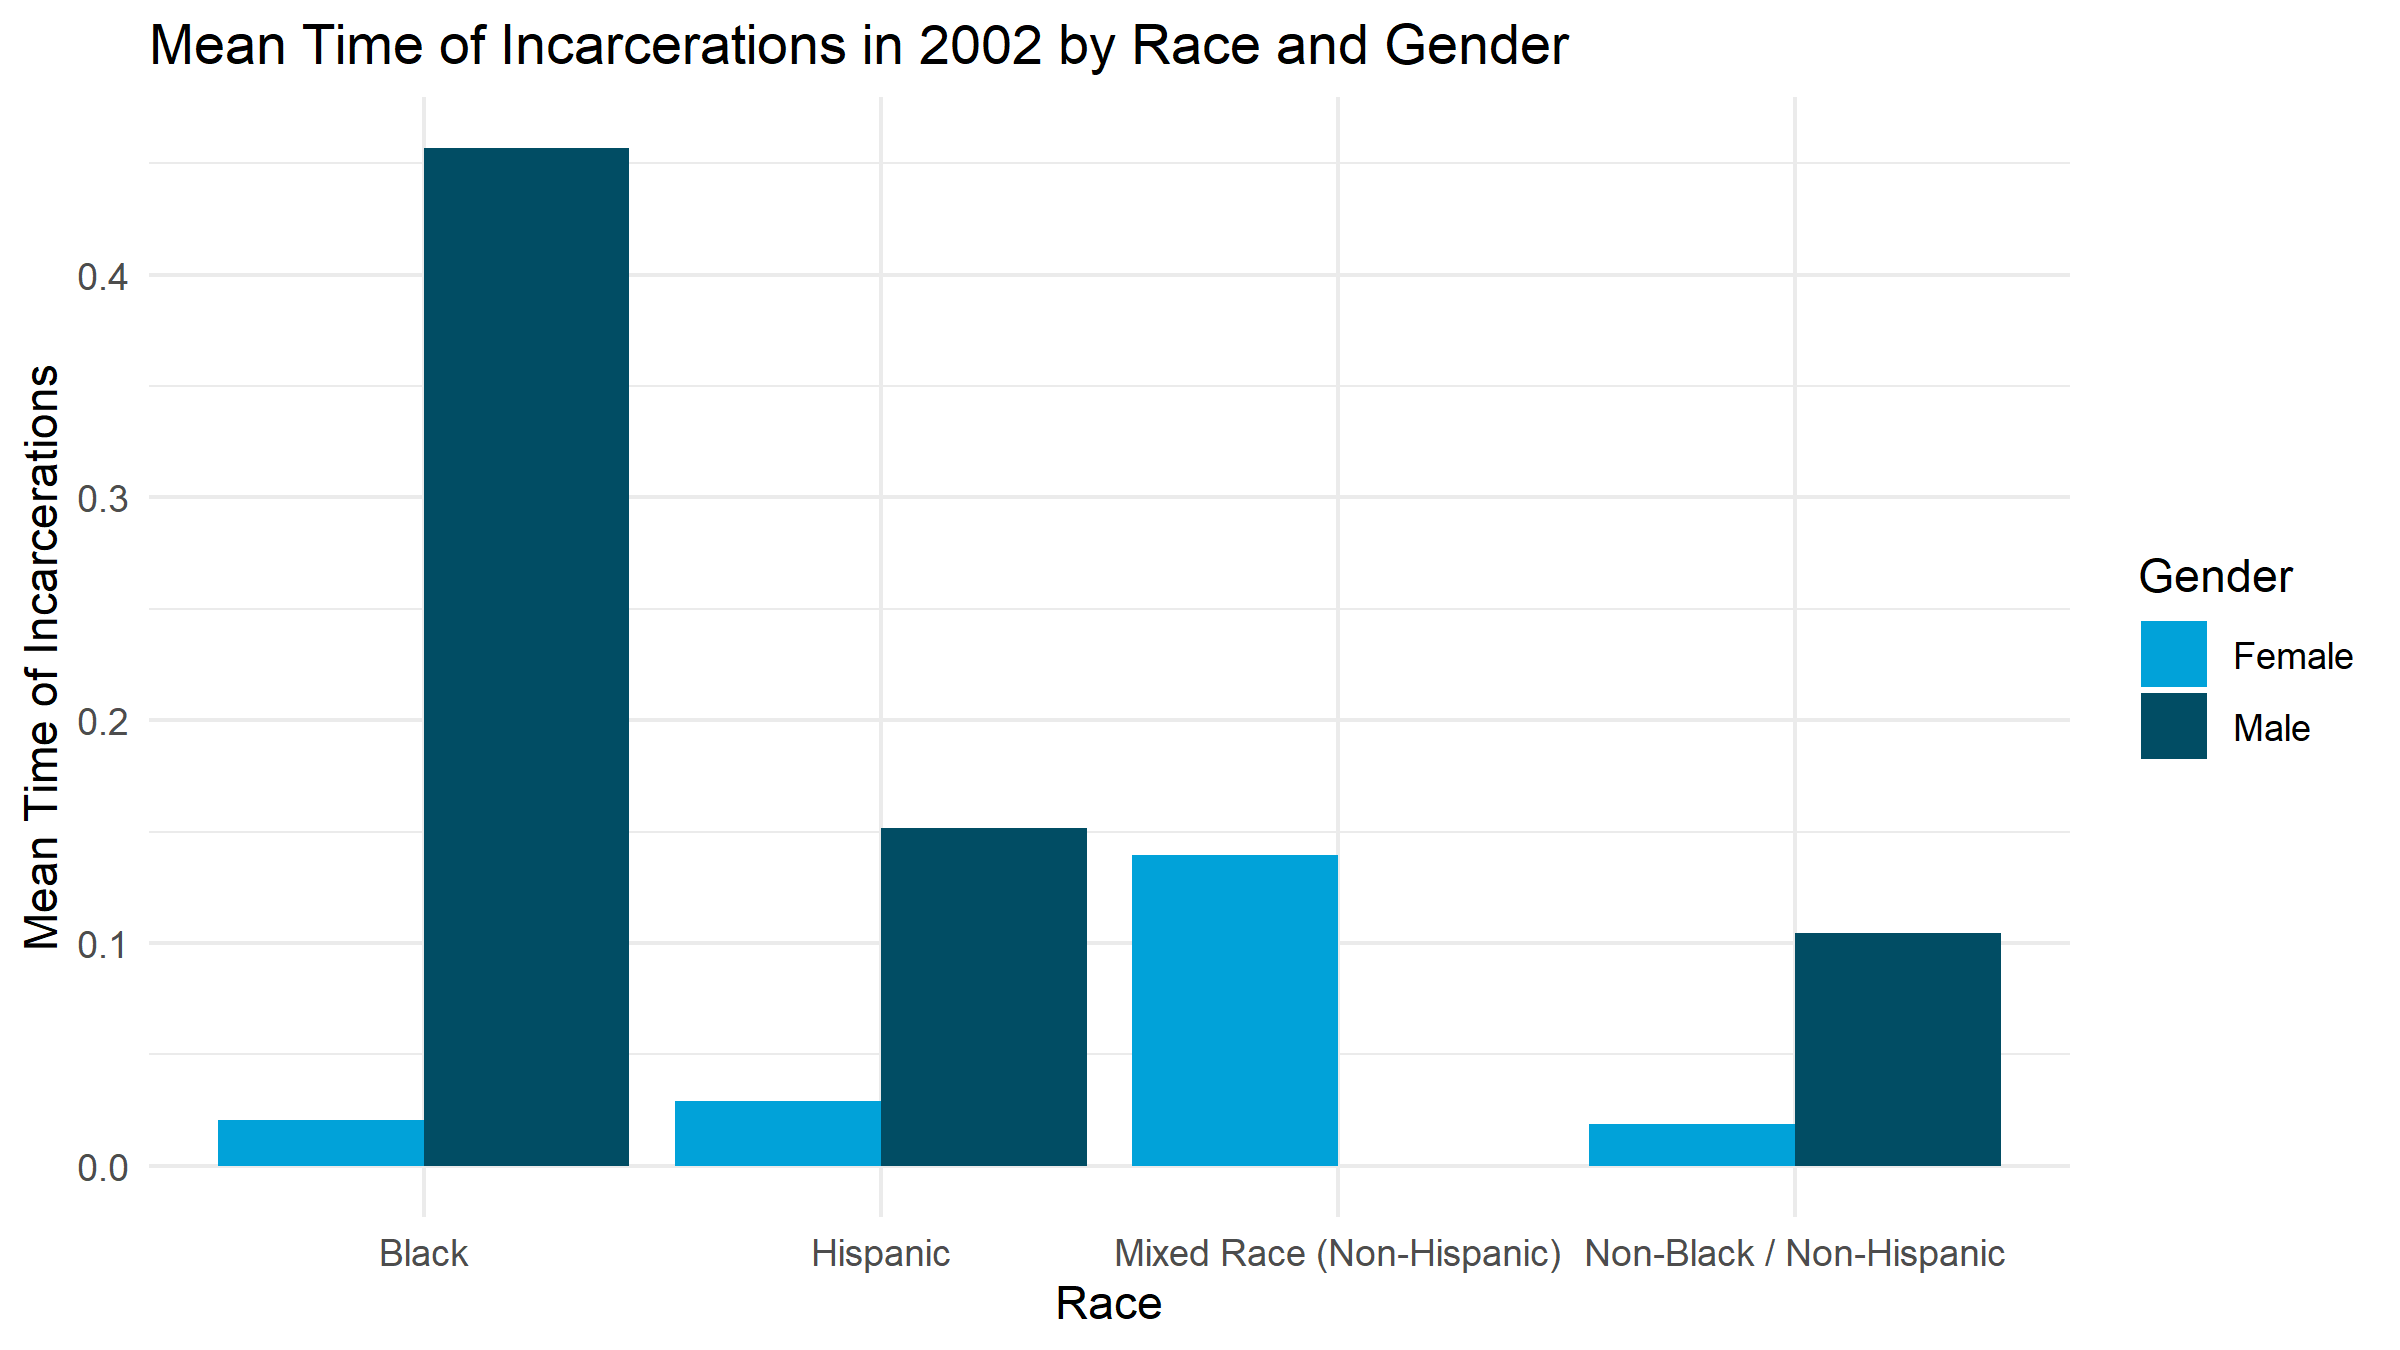
\includegraphics[width=.85\textwidth]{incarcerations_by_racegender}
    \end{center}
    \caption{Mean Time of Incarceration in 2002 by Race and Gender}
    \label{fig:graph}
\end{figure}


Table 1 shows the mean incarceration time categorised by race and gender. Comparing different category shows the same result as the interpretation above. However, these numbers can be given meaning in reality. For example, the mean incarceration time for black females, in this data set, is about 0.02 month. Other categories have similar intuition. These numbers are pretty small, it is because only a little part of interviewee were incarcerated in 2002. 

\begin{table}[H]

\caption{\label{tab:tab:summarystats}Mean incarceration time in 2002 by Race and Gender}
\centering
\begin{tabular}[t]{lrrrr}
\toprule
Gender & Black & Hispanic & Mixed Race Non Hispanic & Non Black Non Hispanic\\
\midrule
\cellcolor{gray!6}{Female} & \cellcolor{gray!6}{0.0205832} & \cellcolor{gray!6}{0.0292208} & \cellcolor{gray!6}{0.1395349} & \cellcolor{gray!6}{0.0186501}\\
Male & 0.4568007 & 0.1514841 & 0.0000000 & 0.1044343\\
\bottomrule
\end{tabular}
\end{table}


Table 2 shows the regression result of a simple metrics model. 

The coefficient of binary variable represents Mixed Race (Non-Hispanic) is significant at 0.1 level, and all other coefficients are significant at 0.01 level. 

These coefficients can provide us with some intuition. Take the coefficient of Hispanic as an example. -0.149 means that holding all else fixed, compared with Black Females, the Hispanic Females spent 0.149 month less in incarceration, in expectation. Here's what the coefficient of sex variable stands for: for Hispanic Males, holding all else equal, they are expected to spent -0.149+0.183=0.034 more month incarcerated. Other categories can be interpreted accordingly.


% Table created by stargazer v.5.2.2 by Marek Hlavac, Harvard University. E-mail: hlavac at fas.harvard.edu
% Date and time: ����, 2�� 16, 2022 - 18:06:17
\begin{table}[!htbp] \centering 
  \caption{Regression Output. Omitted category is Black Females.} 
  \label{tab:regression} 
\begin{tabular}{@{\extracolsep{5pt}}lc} 
\\[-1.8ex]\hline 
\hline \\[-1.8ex] 
 & \multicolumn{1}{c}{\textit{Dependent variable:}} \\ 
\cline{2-2} 
\\[-1.8ex] & Incarcerations in 2002 \\ 
\hline \\[-1.8ex] 
 Hispanic & $-$0.149$^{***}$ \\ 
  & (0.037) \\ 
  & \\ 
 Mixed Race (Non-Hispanic) & $-$0.163$^{**}$ \\ 
  & (0.081) \\ 
  & \\ 
 Non-Black / Non-Hispanic & $-$0.179$^{***}$ \\ 
  & (0.033) \\ 
  & \\ 
 Male & 0.183$^{***}$ \\ 
  & (0.021) \\ 
  & \\ 
 Constant & 0.148$^{***}$ \\ 
  & (0.024) \\ 
  & \\ 
\hline \\[-1.8ex] 
Observations & 8,984 \\ 
R$^{2}$ & 0.014 \\ 
Adjusted R$^{2}$ & 0.013 \\ 
Residual Std. Error & 0.999 (df = 8979) \\ 
F Statistic & 31.172$^{***}$ (df = 4; 8979) \\ 
\hline 
\hline \\[-1.8ex] 
\textit{Note:}  & \multicolumn{1}{r}{$^{*}$p$<$0.1; $^{**}$p$<$0.05; $^{***}$p$<$0.01} \\ 
\end{tabular} 
\end{table} 


\end{document}